This document has been prepared using LaTeX. All figures were created using the open-source software Inkscape and GIMP. The development of this project was carried out entirely within open-source software environments on Linux systems. All Python code associated with this work is released under the GNU General Public License v3 (GPLv3). This serves as evidence that a world without dependence on big software monopolies is possible. 

\section*{Abstract}

Rapid and often unplanned urban growth in seismic regions creates major challenges for disaster risk reduction. In many data-scarce settings, the absence of reliable building inventories limits the ability of local authorities to assess seismic vulnerability, prioritise retrofitting, and plan emergency response. While traditional field surveys can provide accurate results, they are expensive and too slow to apply at city scale. This thesis addresses this gap by proposing a unified computational framework, referred to as the Hybrid Twin, which converts open geospatial data into usable structural engineering information.

The proposed approach combines three main components, remote sensing data, machine learning methods, and physics-informed structural concepts. Recent developments in computer vision, including instance segmentation models such as Mask2Former and SAM2, are used to extract building footprints from high-resolution aerial and satellite imagery with limited manual input. To support this workflow, the GeoImageVision and SeismicBuildingExposure Python packages are introduced, enabling automated dataset generation and the estimation of seismic-related attributes at building level.

A further contribution is the translation of seismic design guidelines from standards such as Eurocode 8, ASCE-7, NTC-23, and the Italian GNDT manual into computational rules. These qualitative criteria are reformulated into measurable geometric indicators which allow consistent estimation of plan irregularity, eccentricity, and compactness across large urban areas. In addition, machine learning models are used to infer structural typologies, such as masonry, reinforced concrete, and adobe, based on footprint geometry and contextual indicators related to construction characteristics.

The framework is evaluated in case studies located in San José, Guatemala City, and Santo Domingo. The results show that the proposed hybrid workflow reduces costs by approximately 84\% to 90\% compared to conventional survey methods, while maintaining consistency comparable to expert assessment. Beyond structural exposure, the framework is extended to urban resilience analysis through accessibility-based evacuation modelling for tsunami scenarios, linking population distribution with evacuation capacity in street networks.

In summary, this thesis shifts seismic risk assessment from static mapping toward more dynamic and predictive modelling. By automating parts of the urban data creation process and improving accessibility to geospatial information, it offers a practical and low-cost approach for improving seismic resilience in data-limited regions. Future work will focus on integrating the tools into unified QGIS plugins, improving model interpretability through explainable AI techniques, and introducing full uncertainty quantification to strengthen reliability in decision-making.

\newpage

\section*{Graphical abstract}

\begin{figure}[htbp]
    \centering
    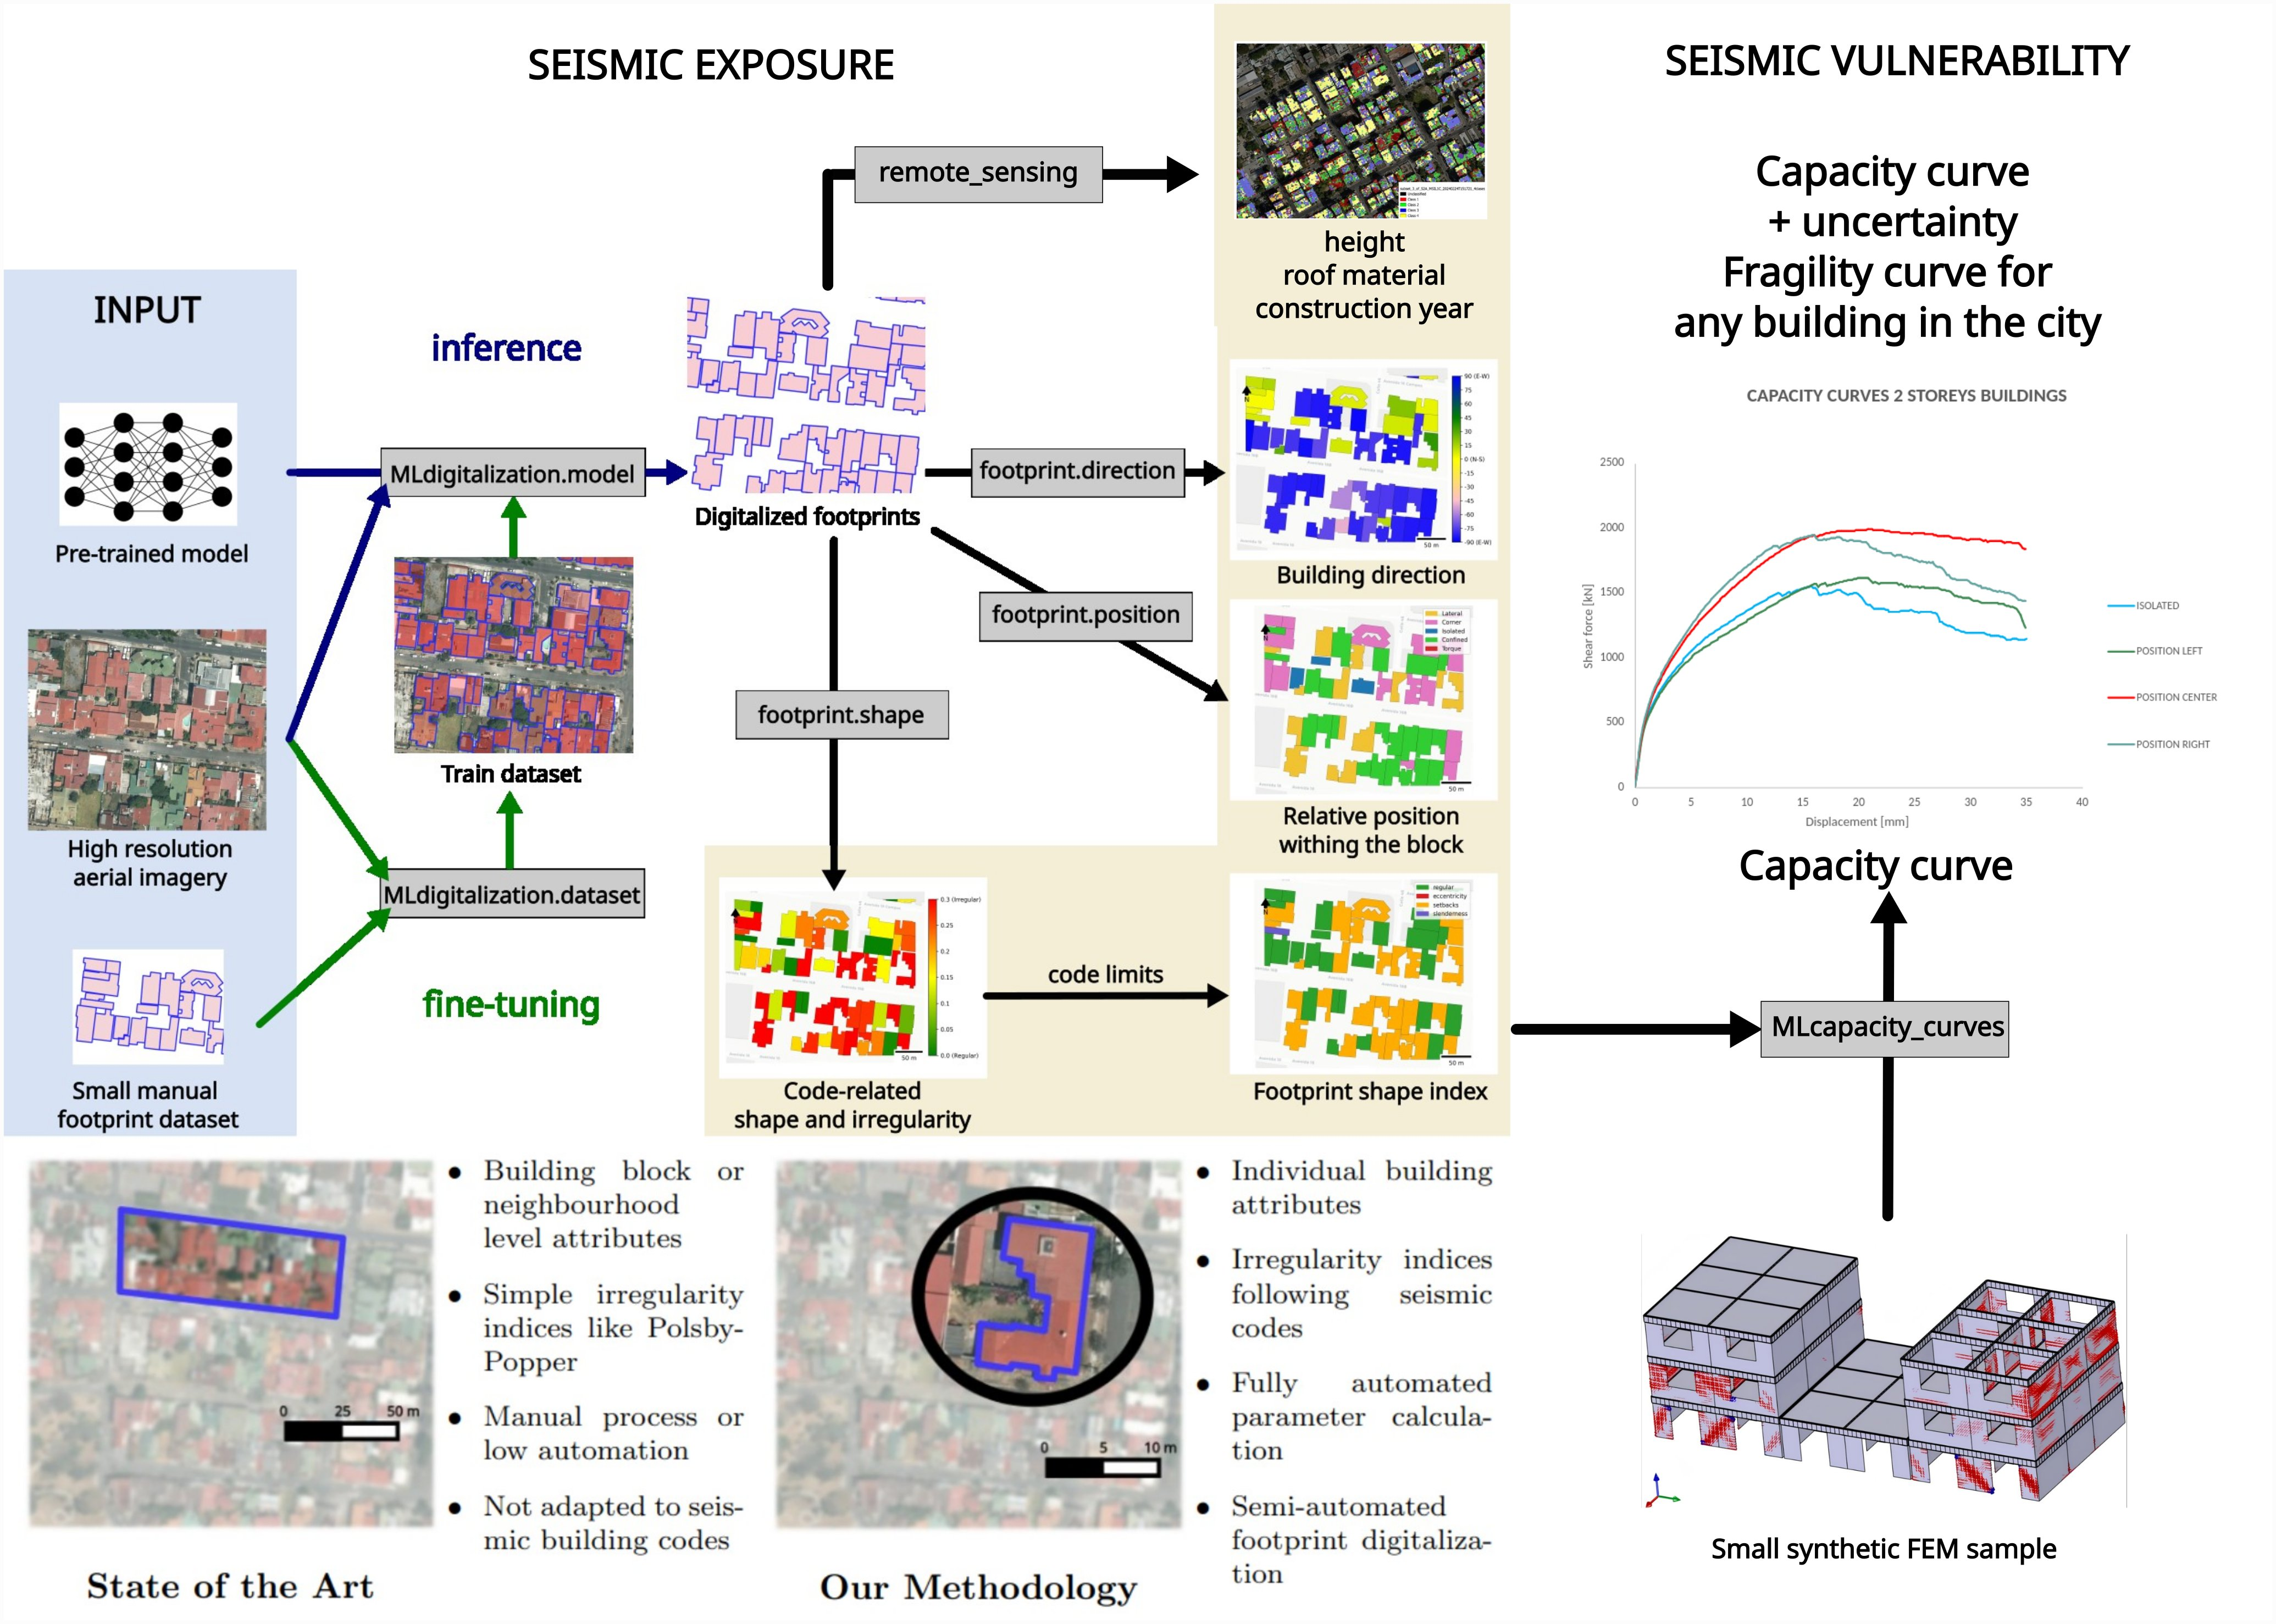
\includegraphics[width=\linewidth]{figures_and_references/complete_workflow.jpg}
    \caption*{Complete proposed hybrid twin workflow and python package modules.}
    \label{fig:complete_workflow}
\end{figure}

\section*{Python packages}

To support the implementation of the proposed framework, four Python packages were developed by the author and made openly available on GitHub. 

\begin{itemize}
    \item \texttt{SeismicBuildingExposure}, which integrates the complete seismic vulnerability workflow. Available at \url{https://github.com/GeomaticsCaminosUPM/SeismicBuildingExposure}.

    \item \texttt{GeoVisionDataset}, designed for constructing training and validation datasets from aerial imagery and open geospatial data for computer vision applications. Available at \url{https://github.com/GeomaticsCaminosUPM/GeoVisionDataset}.

    \item \texttt{GeoVisionModels}, which provides tools for fine-tuning vision foundation models on remote sensing data. Available at \url{https://github.com/GeomaticsCaminosUPM/GeoVisionModels}.

    \item \texttt{UrbanAccessAnalyzer}, focused on computing accessibility metrics, including applications such as the tsunami safety index. Available at \url{https://github.com/CityScope/UrbanAccessAnalyzer}.
\end{itemize}


\newpage